\chapter{Еда и Рецепты}
\section{Как приготовить борщ по классическому рецепту}
\textit{Источник: \url{https://lifehacker.ru/classic-borshcht/}}

В Киевской Руси борщ готовили из съедобных листьев борщевика — отсюда название. Позднее стали варить со свёклой, а с XIX века добавлять картошку.


Сегодня в каждой семье есть свой рецепт борща. В кастрюлю добавляют и фасоль, и грибы, и копчёности, и даже сельдерей. Мы же научим вас готовить идеальный традиционный борщ.

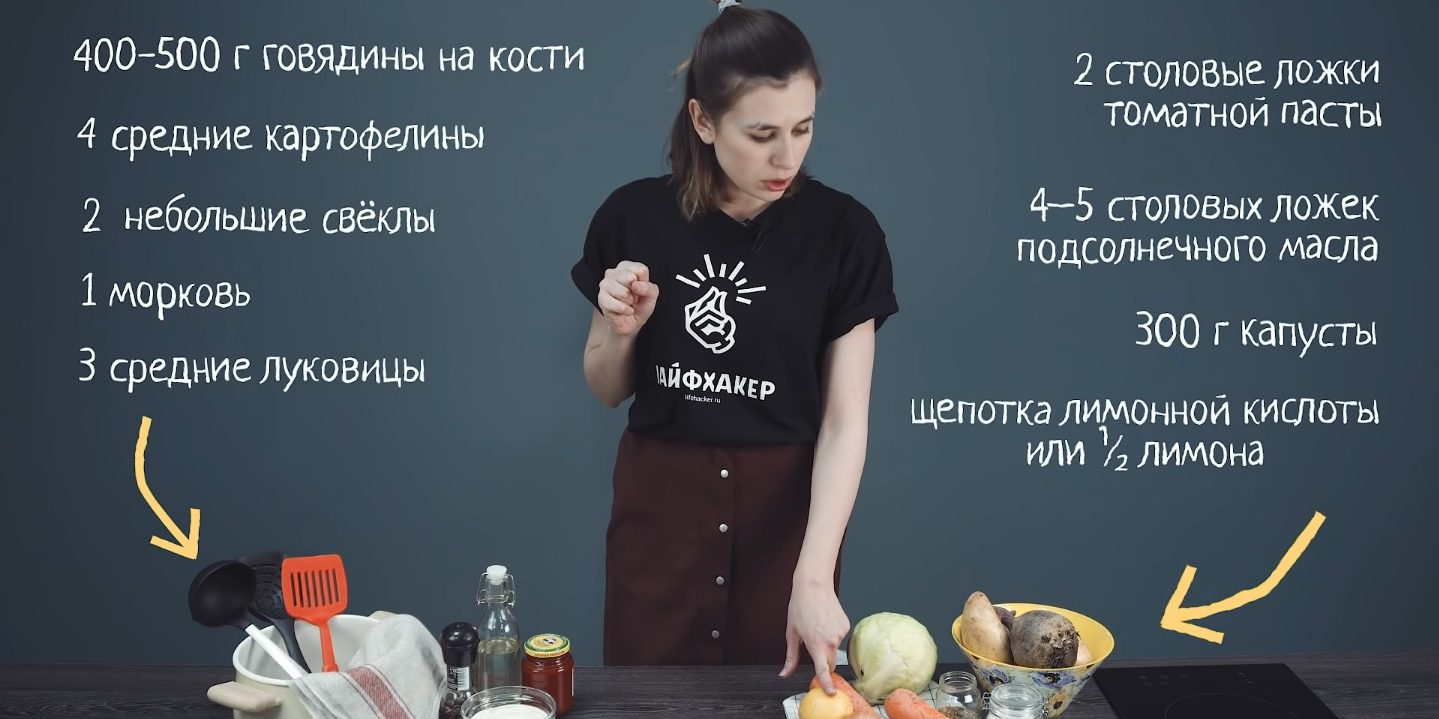
\includegraphics[width=0.75\textwidth]{img/borsch-e1568359200134.jpg}

Для бульона:
\begin{itemize}
    \item 1.5-2 л воды;
    \item400–500 г свинины или говядины на кости.
\end{itemize}


Для зажарки:
\begin{itemize}
    \item 2 небольшие свёклы;
    \item 1 средняя морковь;
    \item 3 средние луковицы;
    \item 4–5 столовых ложек растительного масла;
    \item щепотка лимонной кислоты, немного столового уксуса или ½ лимона;
    \item 2 столовые ложки томатной пасты.
\end{itemize}


Для борща:
\begin{itemize}
    \item 300 г свежей белокочанной капусты;
    \item 4 средние картофелины;
    \item соль — по вкусу;
    \item 1–2 сушёных лавровых листа;
    \item зелень — по вкусу;
    \item 1 зубчик чеснока — опционально;
    \item щепотка молотой гвоздики — опционально;
    \item щепотка молотого чёрного перца — опционально.
\end{itemize}

\textbf{Шаг 1. Сварите бульон.} Налейте в кастрюлю холодную воду, выложите мясо и поставьте на средний огонь. Бульон будет вкуснее, если использовать именно мясо на кости.

Следите за бульоном, перед закипанием снимите пену.

Когда жидкость закипит, накройте кастрюлю крышкой и варите на медленном огне час-полтора.

\textbf{Шаг 2. Сделайте зажарку.}
Вымойте и почистите свёклу, морковь и лук. Свёклу натрите на крупной тёрке, а морковь — на средней. Лук нарежьте небольшими кубиками.

Налейте масло в сковороду, включите средний огонь. Обжаривайте лук и морковь, помешивая, около 5 минут.

Затем выложите свёклу. Добавьте к ней лимонную кислоту, уксус или сок лимона. Благодаря этому борщ будет по-настоящему красным и приобретёт приятную кислинку.

Готовьте зажарку ещё 5 минут. После этого добавьте томатную пасту, перемешайте и оставьте на огне ещё на 5–7 минут.

\textbf{Шаг 3. Соберите борщ.}
Когда бульон сварится, выньте из него мясо. Пока оно остывает, засыпьте в кастрюлю нашинкованную капусту. Через 5–10 минут добавьте нарезанный соломкой или кубиками картофель.

Порядок закладки овощей можно менять. Если капуста молодая, её лучше добавить уже после картошки. Ну или одновременно, если ваш сорт картофеля разваривается быстро.

Пока варится картофель, отделите мясо от кости и нарежьте кубиками. Верните его в суп. Посолите по вкусу.

Добавьте зажарку и перемешайте.

Закиньте лавровый лист и мелко порубленную зелень. Накройте кастрюлю крышкой и варите ещё 5–7 минут.

Для аромата можно добавить в кастрюлю немного измельчённого чеснока, молотой гвоздики или чёрного перца. Оставьте борщ под крышкой настаиваться 5–10 минут.

\textbf{Как подать борщ на стол.} Борщ можно есть сразу после приготовления. Но, как правило, на следующий день он ещё вкуснее.

Добавьте в тарелку сметану и свежую зелень. Если предпочитаете покислее, положите дольку лимона.

Подайте к борщу ржаной хлеб или сдобные булочки, натёртые чесноком. Также блюдо прекрасно дополнят сало и пампушки.


\newpage
\section{Баклажаны Имам Баялды}


 {\it Источник: \url{https://www.gastronom.ru/recipe/46930}}

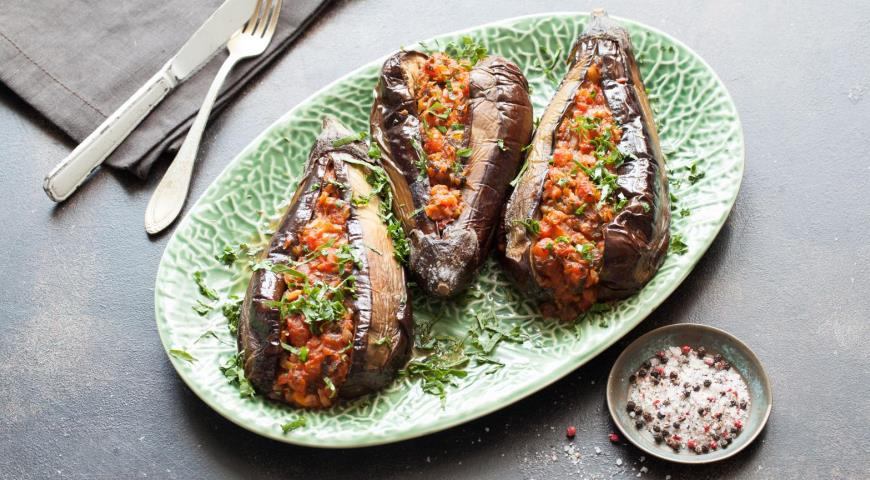
\includegraphics[width=0.75\textwidth]{img/baildi.jpg}

Баклажаны Имам Баялды популярно в турецкой, а также болгарской, армянской, греческой и других кухнях Балканского региона. Название переводится буквально как «имам упал в обморок». А вот причина его падения расходится от легенды к легенде. По одной версии он упал от аромата блюда, по другой – узнав цену. Третья же версия рассказывает о том, что женившись на девушке имам получил в приданное 12 кувшинов лучшего оливкового масла.12 дней девушка угощала мужа баклажанами с помидорами, а на тринадцатый не увидев блюда на столе, имам упал в обморок, поняв, что приданного больше нет.

\textbf{Ингридиенты.} 6 баклажанов (около 900 г);
2 средние красные луковицы;
4 зубчика чеснока;
5–6 веточек петрушки;
1 сладкий зеленый перец;
4 средних помидора;
1 ч. л. сахара (по желанию);
1 ч. л. молотой зиры;
1 ст. л. томатной пасты;
4 ст. л. оливкового масла;
соль;
свежемолотый черный перец.

% ПОШАГОВЫЙ РЕЦЕПТ ПРИГОТОВЛЕНИЯ
\textbf{Пошаговый рецепт приготовления}

Шаг 1. Разогрейте духовку до 220 °С. Застелите противень фольгой или пергаментом и смажьте оливковым маслом.

Шаг 2. Используя овощечистку, срежьте часть кожи баклажанов, чтобы получились широкие полоски. Надрежьте баклажаны вдоль, но не прорезайте их полностью. Посолите баклажаны внутри и снаружи, затем положите их в дуршлаг и оставьте на 30 мин.

Шаг 3. Положите баклажаны на противень и запекайте 20 мин.

Шаг 4.  Очистите лук и чеснок и мелко нарежьте. Измельчите петрушку. У сладкого перца удалите семена и перегородки, нарежьте кубиками. Помидоры надрежьте крест-накрест и положите в миску, залейте кипятком на 2 мин., затем обдайте холодной водой. Снимите кожицу, мякоть мелко нарежьте.
Подпишитесь на рассылку рецептов и советов
Подписаться


Шаг 5. Разогрейте в сковороде 2 ст. л. оливкового масла и обжарьте лук до мягкости. Добавьте перец и чеснок и продолжайте жарить еще 7–10 мин., посолите и поперчите. Положите помидоры и томатную пасту, зиру и петрушку. Если нужно, добавьте сахар. Тушите 5 мин. и снимите с огня.

Шаг 6. Уменьшите температуру духовки до 180 °С. Положите баклажаны в форму для запекания и наполните томатной смесью. Сбрызните оливковым маслом, добавьте 2 ст. л. воды в форму и выпекайте 40–45 мин.

Шаг 7. К концу приготовления баклажаны должны быть практически плоскими, а жидкость в форме должна почти выпариться. Подавайте баклажаны теплым или полностью остывшими.

\textbf{Пошаговый рецепт приготовления}

Шаг 1. Вскипятите 2,5 л воды, посолите и опустите спагетти. Варите пасту до упругости согласно инструкции на упаковке, примерно 6-7 мин. Откиньте на дуршлаг, дайте стечь воде.

Шаг 2. В глубокой сковородке разогрейте оливковое масло и обжарьте нарезанный ломтиками чеснок, 30 сек. Добавьте нарезанную соломкой ветчину и готовьте 3 мин.

Шаг 3. Соедините желтки со сливками и взбейте венчиком. Добавьте соль, свежемолотый черный перец, тертый пармезан и мелко нарезанный базилик, тщательно перемешайте.

Шаг 4. Переложите спагетти в сковородку с ветчиной, перемешайте и прогрейте, 1 мин. Разложите пасту карбонара с ветчиной и сливками в подогретые тарелки и полейте сливочным соусом.






\newpage
\section{Паста карбонара с ветчиной и сливками}


 {\it Источник: \url{https://www.gastronom.ru/recipe/53070}}

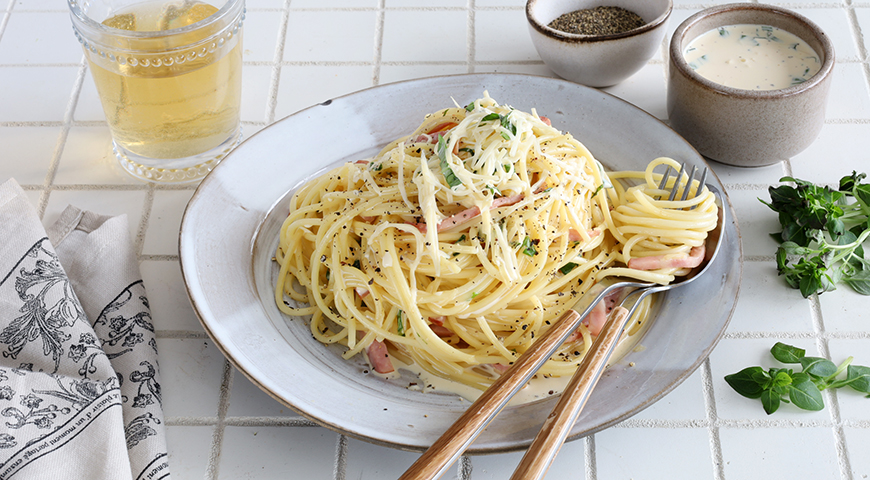
\includegraphics[width=0.75\textwidth]{img/carbonara.jpg}

Паста карбонара с ветчиной и сливками — один из вариантов приготовления этого знаменитого блюда. Поборники традиций, конечно, будут недовольны столь вольным обращением с классикой, однако к подобным кулинарным фантазиям сами итальянцы относятся довольно спокойно. Тем более что паста карбонара, приготовленная по этому рецепту, получается действительно очень вкусной и, как ей полагается, сытной. Сливки придают соусу приятную нежность, которую непременно оценят ваши близкие. Что касается ветчины, мы бы очень рекомендовали использовать сырокопченую: с ней паста карбонара станет значительно вкуснее.

\textbf{Ингредиенты.}
400 г спагетти;
200 г ветчины;
150 мл сливок жирностью 22\%;
2 сырых желтка;
50 г тертого пармезана;
2 ст. л. оливкового масла;
2 веточки базилика;
свежемолотый черный перец;
соль;
2 зубчика чеснока.